% Article about SE abstracts quality (qabstracts) for IEEE Trans. on Software Engineering
\documentclass[10pt,journal,compsoc]{IEEEtran}

\usepackage{cite}
%\usepackage[caption=false,font=normalsize,labelfont=sf,textfont=sf]{subfig}
%\usepackage{stfloats}
\usepackage{url}
\usepackage{hyperref}
%\usepackage{verbatim}
\usepackage{graphicx}
\graphicspath{ {../img} {.} }
\usepackage{balance}
\hyphenation{semi-conduc-tor IEEE-Xplore}

\newcommand{\ifarxiv}[1]{#1}  % activate this for the ArXiv version of the document
%\newcommand{\ifarxiv}[1]{}  % activate this for the journal version of the document

\newcommand{\Plot}[2]{%
	\begin{figure}[htb]%
		\centering\includegraphics[width=\columnwidth]{#1}%
		\vspace{-4mm}\caption{#2}\label{#1}%
	\end{figure}}

\newcommand{\Plotwide}[2]{%
	\begin{figure*}[tbp]%
		\centering\includegraphics[width=\textwidth]{#1}%
		\vspace{-4mm}\caption{#2}\label{#1}%
    \end{figure*}}

\newcommand{\Cb}[1]{\bgroup\scshape #1\egroup}  % typeset a code name
\newcommand{\Prg}[1]{\bgroup\ttfamily #1\egroup}  % typeset commands etc.

\newcommand{\Todo}[1]{\bgroup\bfseries\Large #1\egroup}
\newcommand{\Quote}[1]{\bgroup\itshape ``#1´´\egroup}
\newcommand{\Pseudoquote}[1]{\bgroup\itshape ``#1´´\egroup}
\newcommand{\QuoteCB}[1]{\Quote{#1}}
\newcommand{\Describegroups}{The plots in each group show these different subsets of abstracts:
	all, structured, non-structured, design, empirical, EMSE, ICSE, IST, TOSEM, TSE.}

\begin{document}
	
\title{How (Not) To Write a\\Software Engineering Abstract}

\author{Annie Author1, Bert Author2
\thanks{A. Author1 is with A University, Btown, Ccountry}
\thanks{B. Author2 is with D University, Etown, Fcountry}}

\markboth{IEEE Transactions on Software Engineering}%
{How (Not) To Write a Software Engineering Abstract}

\maketitle

\begin{abstract}  % 100 to 200 words are allowed (but not enforced)
\emph{Background:}
Abstracts are a very valuable element in a software engineering research article,
but not all abstracts are as informative as they could be.
\emph{Objective:} 
Characterize the structure of abstracts in high-quality venues, 
observe and quantify deficiencies, 
suggest guidelines for writing informative abstracts.
\emph{Methods:}
Use open coding to derive concepts that explain relevant properties of abstracts
and identify the archetypical structure of abstracts.
Use quantitative content analysis to objectively characterize abstract structure
over a sample of 500!!! abstracts from five presumably high-quality venues.
Use exploratory data analysis to find recurring issues in abstracts.
Compare the prototypical structure to actual structures to derive
guidelines for producing informative abstracts.
\emph{Results:}
!!!
\emph{Conclusions:}
(1)~Even in top venues, many abstracts are far from ideal.
(2)~Structured abstracts tend to be better than unstructured ones, 
but (3)~artifact-centric works need a different structured format.
(4)~The community should start requiring conclusions that generalize, 
which currently are often missing.
\end{abstract}

\begin{IEEEkeywords}
!!!.
\end{IEEEkeywords}


%========================================================================
\section{Introduction}
\IEEEPARstart{A}{lthough} the abstract is a super important part of any research article\Todo{reference!},
when reading an abstract in software engineering, even in a presumably top-quality venue,
we often feel it is lacking important information or find it difficult to understand at all.

The present article aims at substantiating this impression.


%Ideally, an abstract should 
%situate the work within software engineering,
%motivate and state the issue addressed by it,
%describe the methods applied,
%report empirical results,
%and formulate a useful take-home message.
%With the possible exception of discussing related work,
%this is much the same agenda as for the article itself,
%just with much less detail;
%getting it right is no easy task.


\subsection{Research Questions}

% we use the numbers only in this subsection and the next;
% everywhere else we repeat the question or paraphrase it.
\noindent 
We ask several questions:
\begin{enumerate}
	\item What does a typical well-written abstract look like?
	\item Which deficiencies occur? 
	\item How often?
	\item Do structured abstracts have better quality than unstructured ones?
	\item How should software engineering abstracts be written?
\end{enumerate}
Of these, numbers 1 and 2 should be considered exploratory,
number 4 is hypothesis-driven (we expect a yes), and
the answer to number 5 we consider a conclusion from the answers to the other four. 


\subsection{Research Approach}

No firm expectations regarding questions 1 and 2 exist for engineering articles,
so qualitative methods will have to be used for them:
We start our research by open coding~\cite{StrCor90} in order to derive a vocabulary (a set of concepts or codes)
by which the nature of a particular abstract can be characterized.

We intend to convince even people who are skeptical of qualitative research
regarding our answers to questions 3, 4, and 5 and regarding the need to improve
the quality of software engineering abstracts.
Therefore, we continue the research by performing a repeatable
quantitative content analysis~\cite[Chapter 7]{Krippendorff04} for number 3
on a large sample of presumably high-quality abstracts
and apply an elaborate seven-step approach for maximizing its reliability.

The final stage is the statistical evaluation of the content analysis data,
which is again exploratory and is straightforward in both
the questions it asks and the statistical methdods it uses for answering them.


\subsection{Research Contributions}

Our contributions correspond to the research questions as follows:
\begin{enumerate}
	\item As for the structure of well-written abstracts, we present an ``abstract archetype´´
	  that describes fixed parts of the structure and degrees of freedom. 
	\item We describe and discuss !!! types of deficiency 
	\item We quantify the frequency of each deficiency for the entire sample of abstracts
	  we looked at as well as for 9 different subgroups of interest.
	\item We present convincing data that structured abstracts tend to be better 
	  in several respects.
	\item We provide data-based how-to instructions for abstracts writing for authors
	  as well as guidance for editors and conference organizers.
	  Software Engineering works should use structured abstracts, but
	  need a different and more flexible template than what is used so far.
\end{enumerate}


%========================================================================
\section{Related Work}

There is a considerable literature on research abstracts across disciplines
and we will not attempt to summarize it here.
Instead, we only provide examples of the different major perspectives of those studies
and otherwise focus on what has been done in the software engineering domain.


\subsection{Abstracts Structure}

Swales introduced ``genre analysis´´ as a means for teaching academic reading and writing
especially to non-native speakers in 1990~\cite{Swales90}.
Genres are text types and genre analysis means deconstructing the composition
of texts (of that text type) in terms that help understand the elements in
terms of their syntactical structure, content, role, and interrelationships
(e.g. their relative position within the whole).

For our purposes here, the most relevant idea from genre analysis is the notion
of ``moves´´, which are, roughly speaking, the building blocks used by the writers
for making their overall point.
Several studies have looked at the move structure of research abstracts
in different fields such as 
applied linguistics~\cite{DosSantos96} or
protozoology~\cite{CroOpp06}.
Despite the differences of research content, they find very similar move structures.
For instance,~\cite{CroOpp06} formulates
\begin{quote}
	move 1 situates the research within the scientific community;\\
	move 2 introduces the research by either describing the main features of the
    research or presenting its purpose;\\
	move 3 describes the methodology;\\
	move 4 states the results; and\\
    move 5 draws conclusions or suggests practical applications.
\end{quote}
We found a similar structure (and use it with some extensions)
for empirical works in software engineering, 
but abstracts of artifact-centric works (tool building) do not fit this model and need
an extended one.


\subsection{Abstracts Quality}

Once a ``good´´ structure for abstracts is known, it provides an approach for
discussing the quality of specific actual abstracts.
For instance~\cite{CroOpp06}, where quality assessment is not a main goal,
nevertheless finds that one third of the 12 abstracts studied
is lacking move 2 (stating a purpose).

Several studies have, however, put quality assessment at their center,
most often in subfields of the biomedical domain.
Many such studies comprise articles of a homogeneous nature:
all randomized controlled trials (controlled experiments).
This allows formulating very specific expectations what information should be
presented in an abstract and allows performing the analysis in checklist fashion.
In this manner,
\begin{itemize}
  \item \cite{DupKhoLeb03} used a 30-item checklist on 197 abstracts in clinical dermatology
     for computing a 0-to-1 score and found mean scores between 0.64 and 0.78 for their various subgroups.
  \item \cite{ShaHar06} used a 29-item checklist on 100 abstracts in dental medicine
	 and found a mean score of only 0.54.
     % suggests an 8-move structure for structured abstracts: 
     % objective, design, setting, patients, interventions, outcome measure, results, conclusion.
     % per-move deficit rates are not reported.
  \item \cite{} used a !!!-item checklist on !!! abstracts in !!!field
	 and found !!!\% of them to have deficiencies,
\end{itemize}


\subsection{Structured vs.\ Unstructured Abstracts}

In many cases, and in particular in those parts of the biomedical domain 
where controlled experiments are the norm, quality-oriented studies do not study
quality in general.
For instance neither~\cite{DupKhoLeb03} nor~\cite{ShaHar06} reports
which of their items are missing most frequently.
Rather, their research question is the relative quality of structured abstracts
versus unstructured ones. 
And in almost all of those cases, including~\cite{DupKhoLeb03} and~\cite{ShaHar06},
the answer is: structured abstracts have fewer quality issues.

Such research can be highly influential.
For instance,~\cite{HarSydBlu96} 
% https://journals.sagepub.com/doi/epdf/10.1177/016555159602200503
is cited in the CONSORTS report~\cite{MohHopSch12},
which defines reporting guidelines for controlled experiments and has about
10000 citations.

!!!Budgen work!!!


%========================================================================
\section{Methods}


\subsection{Overview}

Our study is a full-blown content analysis in the sense of Krippendorff~\cite{Krippendorff04}:
not just a counting exercise with a fixed codebook, 
but rather an iterative codebook development before (and during) the counting
and an extensive abductive inference exercise after the counting.

It can be conceptualized as consisting of four widely overlapping stages or phases
as shown in Figure~\ref{qabstracts_timeline_commits}:
%
\Plot{qabstracts_timeline_commits}{%
	Timeline of the main study phases and their individual events.
    Each character's x-coordinate represents the time of a git commit.
    The vertical scattering is added for legibility only and is not meaningful.}
%
Codebook development, which started first and is described in Sections~\ref{meth_codingrules}
and \ref{meth_codebook},
defined the rules and target concepts of the counting.
Training was for developing a joint understanding of the codebook and also contributed
greatly to the codebook's early evolution;  
it is described in Section~\ref{meth_training}
Coding worked on a large sample of abstracts from top-quality venues described in 
Section~\ref{meth_sample} and produced the count data subsequently used in the statistical analysis.
Coding is described in Section~\ref{meth_coding}.
Statistical evaluation 

Overall, we consider our study to be a qualitative one, but note that the middle two elements,
coding and statistical evaluation,
are compatible with a positivist epistemology (with ``objective´´ results) so that 
the final interpretation is done on a solid quantitative foundation.


\subsection{Data Availability}

We publish not only the outcome of our study, but also most parts of its development and
execution history in full detail: as a git version respository.
It includes all versions of the 
codebook, handling procedure, coded abstracts, Python scripts for automation,
Python scripts for tabulations and plots, and the manuscript of this article.
Find it at \url{https://github.com/serqco/qabstracts/}.


\subsection{Coding Rules}\label{meth_codingrules}

Besides the definition of the content categories (codes),
our codebook contains global rules for the coding that can be summarized as follows: 
we code by sentence; 
we prefer single codes per sentence over multi-codings; 
for chosing a code, we act like readers and consider only what we have seen before plus 
one sentence forward context when needed and only when needed; 
be friendly and avoid coding negative properties whenever an alterative, more positive 
interpretation is plausible as well.


\subsection{Codebook Development}\label{meth_codebook}


\subsubsection{\Cb{background, objective, method, result, conclusion}}

The codebook was initialized with concepts for the five sections commonly used 
in a structured abstract\footnote{In Krippendorfs terminology, this is an ``established theories´´ justification
of analytical constructs~\cite[Section 9.2.3]{Krippendorff04}.}: 
\Cb{background, objective, method, result, conclusion}.
These represent, respectively: context information, the study goal or question, 
empirical approach, empirical outcomes, and a take-home message that generalizes beyond the results.

Each code is defined by a short verbal explanation.
For example the definition of \Cb{method} reads
\QuoteCB{information about the approach or setup of an empirical (or possibly purely mathematical) study.}.
The initial definitions were made more and more precise and unambiguous by later
codebook refinements.
For example for \Cb{method}, the part \QuoteCB{(or possibly purely mathematical)} was initially not present
and was added when we encountered the first of those (very few) purely mathematical studies
during the coding process and were confused which code was appropriate for some sentence.
To help disambiguation, a few of the definitions need to be much longer than the above.


\subsubsection{Artifact-centric studies: \Cb{design}}\label{design}

In a phase internally called ``prestudy´´, the codebook was then refined and extended
based on coding attempts for a stratified sample of 20 abstracts from ICSE 2021.
% we used every 7th article, which constitutes stratification by virtue of the
% topic-centric session blocks in which the program is arranged.
We quickly recognized that additional codes were 
needed\footnote{In Krippendorfs terminology, this is an ``expert knowledge and experience´´ justification
    of analytical constructs~\cite[Section 9.2.2]{Krippendorff04}:
    As software engineering researchers, we recognize when a sentence makes a different kind
    of contribution to an abstract than can be described by existing codes,
	and we are able to define what kind of contribution it is.}.
Most importantly\footnote{For brevity, we leave rare or unimportant codes out of the description.}, 
many software engineering articles do not predominantly talk about
an empirical study, their focus is the design of some artifact, most often a tool,
sometimes a method or something else.
Much of the abstract is then spent on design considerations, design decisions,
techniques applied in implementation, and so on.
Such artifact-centric studies, although they also usually contain an empirical study,
are very different in nature from purely empirical studies; 
we therefore introduced the code \Cb{design} to mark such material.
\Cb{design} has the longest definition of all our codes: 170 words.

We call the articles that contain at least one \Cb{design} code in their abstract
``design works´´, the others ``empirical works´´.


\subsubsection{Refinements: \Cb{gap, summary, fposs} etc.}

At various later points during the work, we recognized a need for more granular coding
in order to capture differences in abstract writing we wanted to measure.
This led to the splitting of existing codes and the introduction of additional ones.
We then reworked existing codings to use the new codes consistently throughout.

The most important cases of such additional codes are these:
\Cb{gap} sentences state what is unknown or not yet possible.
\Cb{summary} sentences summarize several results, but do not provide new information.
In contrast to a \Cb{conclusion}, a summary statement does not generalize beyond the immediate results.
\Cb{fposs}, \Cb{fneed}, \Cb{fwork} sentences occur at the end of abstracts.
They state what future work is now possible, needed, or planned-by-the-authors.

% TODO: examples of gap, summary, fposs, conclusion


\subsubsection{Subjective additions: \Cb{:i, :u, :hype}}

The codes described so far aim at codifying repeatable properties,
where several well-trained coders will come to the same result with high probability.
In addition, we defined a number of suffixes for codes, by which coders can provide
additional information for which the expectation of agreement is much lower.
These are also not neutral, like the codes themselves, but all describe some 
kind of deficiency.
The most important of these suffixes are the following:

Informativeness gaps are spots in a sentence where the coder desired to know
additional detail that is presumably available to the authors and 
that can presumably be provided in very little space.
Example (from LiuFenYin22): 
\Quote{To evaluate DeepState, we conduct an extensive empirical study on popular datasets 
and prevalent RNN models containing image and text processing tasks.}
This sentence was coded as \Cb{method:i2}, because the coder asked himself
\Quote{How many datasets? How many RNN models?}
The answers are both given in that article's Table 3: Four datasets, three models.
The authors could and should have given that information in the abstract.

Understandability gaps are spots in a sentence where the coder finds his usual intuitive 
half-understanding of a term used in the abstract insufficient for understanding
the abstract overall.

\Todo{example of :u1}

The \Cb{:hype} suffix marks statements that praise the article far more
than warranted, often by using exaggerated adverbs such as ``extremely´´.


\subsubsection{Codes for announcements: \Cb{a-*}}

Sometimes, statements do not merely have informativeness gaps,
they provide no concrete information at all.
We call such statements announcements (because their presence insinuates there will
be information about this in the article body) and provide extra codes for them.

For example, here is a real method announcement from BesMarBos22:
\Quote{As a second step, this study sets out to specifically
  provide a detailed assessment of additional and in-depth analysis of technical debt management strategies based
  on an encouraging mindset and attitude from both managers and technical roles to understand how, when and by
  whom such strategies are adopted in practice.}
So many words, yet we learn nothing about how 
the assessment\footnote{Also, the sentence appears to be broken in that part.} 
or the analysis work.

Here is a results announcement from FlyChaDye22:
\Quote{Based on those results, we then used the Boa and Software
  Heritage infrastructures to help identify and quantify several sources of dirty Git timestamp data.}
The first part is \Cb{method}, the second should have been \Cb{result},
but, alas, we learn nothing about those sources' nature or number or impact.


\subsubsection{Codes for headings: \Cb{h-*}}

We also have codes for the headings used in structured abstracts.
These codes are conceptual, i.e., for instance 
\Quote{Aim:}, \Quote{Goal:}, \Quote{Objective:}, \Quote{Question:}, and their plural forms
would all be coded as \Cb{h-objective}.
Likewise, there are \Cb{h-background}, \Cb{h-method}, and so on.
We recognize structured abstracts by the presence of such a heading code.


\subsection{Training}

The training phase (internally called ``prestudy2´´) served two purposes:
Finding/repairing deficiencies in the codebook,
and arriving at a joint interpretation of it across the four coders 
(the four authors\footnote{Four more people were involved in the training phase at some
  point but did not eventually join the study.})
As you can see in Figure~\ref{qabstracts_timeline_commits},
the training phase extended over almost half a year and triggered
the majority of the codebook improvements.

In the training phase, we perfected the mechanics of the coding process
described below, in particular the very useful \Prg{compare-codings} script
and email routine,
and generally formed as a research team.


\subsection{Sample}

We decided not to aim for a broad selection of all software engineering research,
but rather concentrate on what is presumably the highest quality material:
The ICSE technical research track,
the three journals allowed for journal-first presentations at ICSE
(Empirical Software Engineering EMSE, 
ACM Transactions on Software Engineering and Methodology TOSEM, 
IEEE Transactions on Software Engineering TSE).
Since we expected to find that structured abstracts had better quality
than unstructured ones, we added a fifth venue that required structured abstracts:
Information and Software Technology (IST, an Elsevier journal).
IST has published many very good systematic literature reviews and methods works,
but is not \emph{generally} considered a top-quality venue.

We wanted to draw a random sample of 100 articles per venue from the
2022 volumes, but found that TOSEM has published only 86 articles per year,
so we ended up at 486 articles initially.
A few of those later had to be removed because they were other things,
often editorials.
Furthermore, we eventually did not need quite as much data for answering our
questions and stopped coding after !!! abstracts.
Still, ours is the largest manual study of abstracts we know of.

Volume downloading, sampling, and abstract extration into publishable 
and annotation-ready text files were all done automatically by the
retrievelit\footnote{\url{https://github.com/serqco/retrievelit/}},
select-sample, and prepare-sample scripts, respectively.


\subsection{Coding process}

\noindent
We code each abstract twice, by so-called coders A and B.\ 
Abstracts are held in text files in separate directories \Prg{abstracts.A} and \Prg{abstracts.B}.
Each sentence is followed by a line containing \Prg{\{\{\}\}} and into this pair of
double braces the coders will enter their codings,
such as \Prg{\{\{method,result:i2\}\}} for a complex sentence that contains substantial
amounts of method information as well as results with two informativeness gaps.
We batch the coding in blocks of 8 abstracts each.
The procedure, coordinated via git, is best explained by example, 
which we do in the following two subsections. 


\subsubsection{Coding}

1. When Lloyd wanted to code a block of abstracts on 2023-05-26,
he found the next available block to be Block 17 B.
(Lutz had coded Block 17 A previously.)
Lloyd reserved the block in the coordination file \Prg{sample-who-what.txt}
and performed the coding.

2. He then ran \Prg{check-codings} to test his codings (for the occasional typo etc.)
against the codebook and corrected the mistakes, if any.

3. He then ran \Prg{compare-codings} to compare his codings against Lutz'.
This script creates one report block for each sentence where the codings
of coders A and B are not compatible.
Compatible means: Differing at most in the subjective suffixes, but not in the codes
(and not by more than one in the numbers of informativeness gaps and understandabity gaps).
If Lloyd found a report block where Lutz' coding was obivously correct and his own
obviously wrong, he would simply correct his coding.

4. He would then commit his coded abstracts into git.


\subsubsection{Handling disagreements}

5. For the remaining report blocks, Lloyd would write an email to Lutz explaining his reasoning.

6. Lutz would read through that email and categorize the report blocks into the following cases:
a) Lloyd's coding is obviously correct, Lutz' own is a simple clerical error.
Lutz would correct his coding and respond accordingly.
Figure~\ref{email-MeyAlmKel22.png} shows such a case.\\
b) Lutz finds Lloyd's coding clearly incorrect. 
He would respond with an explanation why he thinks so.\\
c) Lutz finds Lloyd's coding acceptable, but his own coding preferable.
He would respond with an explanation of his reasoning and suggest that Lloyd
either adjust his coding or add an \Cb{:ignorediff} suffix to it.
This suffix silences the \Prg{compare-codings} script for this particular report block,
so that the coding difference is now officially accepted.\\
d) Lutz finds his own coding acceptable, but Lloyds preferable.
He would either adjust his coding or add an \Cb{:ignorediff} suffix to it
and respond accordingly.\\
e) Lutz finds both codings equally acceptable.
He would add an \Cb{:ignorediff} suffix to his own
and respond accordingly, explaining is reasoning.\\

\begin{figure*}[tbp]%
	\centering\fbox{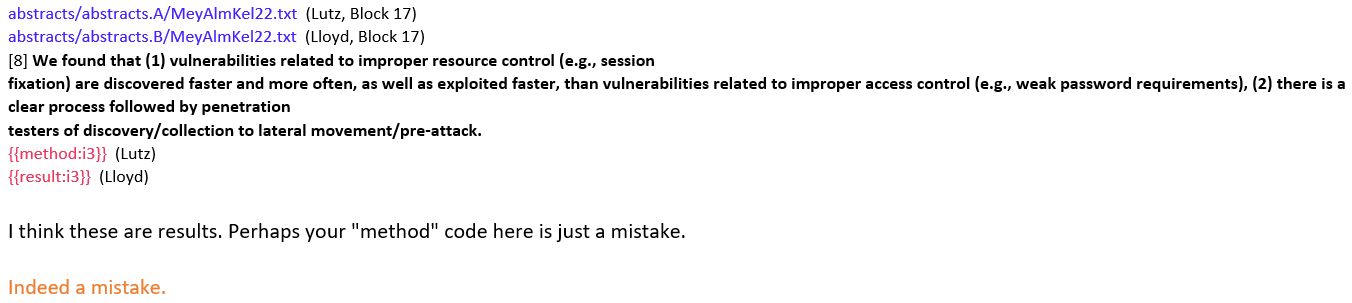
\includegraphics[width=0.95\textwidth]{email-MeyAlmKel22.png}}%
	\vspace{-2mm}\caption{Excerpt from Lutz' response email during the disagreements handling
	  for Block 17: 
	  Report block from the \Prg{compare-codings} script at the top,
	  text line from Lloyds first email in the middle,
	  Lutz' response below.
	  This one was a simple case; 
	  sometimes several lines of text are provided by each coder.
	  Overall, Lloyd's first email contained report blocks for 9 disagreements
	  in 4 abstracts, both typical numbers.}\label{email-MeyAlmKel22.png}%
\end{figure*}

7. Lutz would commit his corrected abstracts and send the response email.

8. Lloyd would read the response email and usually act on it to finish the handling of 
Block 17.
Only very rarely would he disagree with something to a degree that would make
another round of emails necessary.


\subsubsection{Effect of this procedure}

Most content analyses code most material only once, 
then code a random subsample twice, 
compute some coefficient of agreement, 
report it as a measure of good-enough coding quality,
and that's that.

In contrast, our above-described procedure has two effects:
\begin{enumerate}
	\item It maximizes the quality of the coding.
	  Very few clerical errors will have managed to escape our discussion process
	  and the definitions of all codes that are sometimes difficult to tell apart
	  have been refined until they were very mature.
	\item It finds all those spots in the sample where the abstracts are so convoluted
	  or strangely formulated that even our careful code definitions do not lead
	  to a canonical judgment.
	  These spots should clearly be considered to be badly written -- which is great,
	  because that is what our study is interested in.
\end{enumerate}


\subsection{Statistical Evaluation}

The difficult part of our statistical evaluation is asking the right questions;
our data provides a lot of possibilities.
In contrast, the actual statistical techniques are simple and straightforward:
Mostly tabulations of counts or percentages, bar plots, and box plots.

We mostly refrain from performing significance tests or computing confidence intervals,
because most analyses are exploratory, not driven by specific expectations or theories.
The one exception from this rule is the comparison of structured versus unstructured abstracts.

!!!Verbal terms for frequencies: 
rare (less than 5\%),
not rare (5-20\%),
common (20-35\%),
frequent (35-50\%),
dominant (over 50\%).


\subsection{Interpretation}

!!!Driven by research interest; grounded as far as possible.
Makes use of impressions not captured in the data.
Choice of examples reflects those.


%========================================================================
\section{Results}

\subsection{Length and Readability}

Typical abstracts (the middle half) are 200 to 290 words long
and 8 to 14 sentences long.
Structured abstracts tend to be longer than unstructured ones.
\ifarxiv{See Figures \ref{boxplots_words} to \ref{boxplots_avg_wordlength} for details.}
The official word limits of 
150--250 for EMSE,
maximum 300 for IST, and
recommended maximum 250 for TSE
are disobeyed by more than a quarter of all articles for each of these three venues.

The Flesch-Kincaid readability score is a widely used metric that judges
readability based only on the number of words per sentence and the number of 
syllables per word. 
Values under 30 represent graduate-level difficulty,
under 10 extreme difficulty for native speakers.
Considering that most community members are not native speakers of English,
we judge 20 to 30 to be a range suitable for researcher audiences and so 
we call anything over 30 ``good´´, 
20 to 30 ``normal´´, and 
under 20 ``overly difficult´´.

See Figure~\ref{boxplots_fkscore} for the results:
only about 10\% of all abstracts have good readability,
less than 40\% have normal readability,
and a majority is overly difficult --- one quarter is even below 10!
ICSE is a bit better than the other venues,
TOSEM is worse.

\Plot{boxplots_fkscore}{%
	Flesch-Kincaid 'reading ease' readability score, higher is better.
    Values under 50 are considered difficult to read (college-level material).
    Under 30: very difficult to read (graduate level, acceptable for abstracts).
	Under 10: extremely difficult to read (overly difficult).
    Differences between subgroups are modest. 
	ICSE is best (mean 20), TOSEM is worst (mean 13).
    Structured abstracts are just as difficult as nonstructured ones
    if one ignores the ``Methods:´´ etc. headings as we did here.
}


\subsection{Design Articles vs. Empirical Articles}

We described the idea of the \Cb{design} code in Section~\ref{design}.
But many empirical works involve some artifact design as well,
so how is the discrimination made?
That depends on how the authors phrase their goal in their
\Cb{objective} statement.
Consider the following goal statements:

!!!

The first puts the artifact at the center, so this is a design work.
The second puts empirical results at the center, so this is an empirical work
and the design code will not be used for them.
Artifact design discussion will then usually be coded as \Cb{method} instead. 
Mixed cases are rare and then the coders will decide which aspect has more weight.

In design works, a large fraction of the abstract will be devoted to
describing design considerations for that artifact;
in our data: typically 16\% to 34\% of the words.
The empirical study, which usually exists as well, then usually has a mere 
supporting role (validating the claims made in the artifact discussion)
and is correspondingly given less space: 
7\%--15\% (versus 12\%--23\%) for description of empirical method,
12\%--24\% (versus 18\%--32\%) for description of empirical results.


\subsection{The Abstracts Archtetype}

Compared to the content structure assumed by the usual formats of
structured abstracts, our codebook is more fine grained;
the \Cb{design} code is but one example. 

During our sensemaking process, we had a number of insights regarding
how a well-written abstract ``ticks´´, which we eventually distilled into
the following template, which we call the software engineering abstracts archetype:

\begin{enumerate}
\item An abstract consists of three parts, in this order:
   \emph{Introduction}, \emph{Study Description}, and \emph{Outlook}. 
\item Two turning points connect the three parts:\\
   a) A statement of the study goals (\Cb{objective}) connects \emph{Introduction} 
      to \emph{Study Description}.\\
   b) A generalizing statement ("take-home message", \Cb{conclusion}) 
     connects \emph{Study Description} to \emph{Outlook}.
\item The \emph{Introduction} first introduces the topic area of the study and what is known (\Cb{background})
   and then may or may not point out a gap in knowledge (\Cb{gap}).
\item For an empirical article, the \emph{Study Description} begins with
   method description (\Cb{method}), followed by results description (\Cb{result}).
   Sometimes, this sequence occurs twice in a row, very rarely more.
\item For a design article, design description (\Cb{design}, see below) precedes the structure
   described in the previous point.
\item Occasionally (but infrequently), \emph{Study Description} will end with a study summary (\Cb{summary}).
\item After the \Cb{conclusion}, the \emph{Outlook} talks about future research and states 
   what could now be done (\Cb{fposs}, for future possibilities),
   what should now be done (\Cb{fneed}),
   what the authors themselves intend to do (\Cb{fwork}), or
   what is still not known (\Cb{fgap}).
   Several statements of each type may occur, in no particular order.
\end{enumerate}

The archetype describes all variants of abstracts that have a natural train of thought,
so any deviation will lead to a less easily understandable abstract.

!!!example(s)?


\subsection{How Not To: Missing Elements}

Given the archetype, one way to approach an analysis of abstracts quality is to ask
how often key parts of an abstract are missing entirely.
This is shown in Figure~\ref{zerofractionbar_xletgroups_topicmissingfractions}.

\Plotwide{zerofractionbar_xletgroups_topicmissingfractions}{%
	How often is a topic not present at all in an abstract?\\
	\Describegroups}

The often-missing parts \Cb{gap} and \emph{Outlook} are clearly optional, 
so it is not a problem that they are often not present.
\Cb{background} and \Cb{objective} are hardly ever missing.

\Cb{method} and \Cb{result} are sometimes missing (and this is a problem), 
but never in structured abstracts.
This is the first of several indications that structured abstracts are indeed a good idea.

The shocking part of this analysis is \Cb{conclusion}, which ought to be present
as the key take-home message in any abstract, but is in fact missing in more than
half of all -- yet again very rarely in structured abstracts\footnote{Note that 
  the prompt of having to write something after a "Conclusion:" keyword
  alone cannot guarantee this: 
  The statement put there can be (and sometimes is) something else e.g. a \Cb{result} statement
  or \Cb{summary}.}


\subsection{How Not To: Convoluted Trains of Thought}

Leaving out important parts from an abstract is not the only way for wrecking
the abstract's value, however.
There are also abstracts where the train-of-thought is so convoluted
that they become difficult to read.

For quantifying this, we map each abstract to a short sequence of letters,
where each letter stands for a contiguous stretch of sentences in the abstract
that have the same content type; the letter designates that content type.

For instance, an abstract that follows a minimal incarnation of the Archetype
for an empirical article would be encoded as bomrc, which stands for
the content types sequence background, objective, methods, results, conclusion.

The full list of abstracts structures is too long to show it here.
It has 95!!! entries for empirical articles and 122!!! entries for design articles.
Most of these have only one or two instances, though; 
we restrict ourselves to the types that occur with higher frequency here. 
Note that a frequency of e.g. 2.5 simply means that the two coders did not agree.
The results are shown in 
Figure~\ref{ab_topicstructure_freqs_empir} for empirical articles and
Figure~\ref{ab_topicstructure_freqs_design} for design articles.

\Plot{ab_topicstructure_freqs_empir}{%
  The frequency of different trains-of-thought in the abstract for empirical articles.
  The label is a string of stretch-code characters:
  b-ackground, g-ap, o-bjective, d-esign, m-ethod, r-esult, s-ummary, c-onclusion, O-utlook.}
\Plot{ab_topicstructure_freqs_design}{%
  The frequency of different trains-of-thought in the abstract for design articles.
  Same characters as before, except that d can now in fact occur.}

\subsubsection{Empirical articles}

Let us start with the simpler empirical articles.
We see that the most sensible structures are also the most frequent (bars 1, 2, 3):
Archetypical with or without a \Cb{gap} statement, perhaps with an \emph{Outlook}.
But from bar 4 on, the abstracts are more or less pathological:
The first few are mostly missing a conclusion, later on (not shown in the figure)
follow all kinds of curious structures such as, to pick an admittedly extreme case,
bgomrcsrsc: two conclusions, two summaries, summary after conclusion.

\subsubsection{Design articles}

It naturally gets worse for the design articles with their more complicated structure:
Even the top two structures are missing a conclusion
and we find complex repetitive structures starting at bar 5.
Not all of these are automatically bad. 
In particular, having two small empirical studies, resulting in a nice bgodmrmrc structure,
can make a lot of sense for the reader.
But this has its limits: An abstract with structure bodmrmrmrmr is overloaded.
It can also easily get out of hand, as confirmed by the examples bobdrmrmr and bomdmrmrmrsmrc.

\subsubsection{Structured abstracts}

Today's conventions for structured abstracts may be a bit restrictive
(e.g. by not accomodating the useful mrmr substructure), 
but they result in more orderly abstracts:
There are only 27!!! different abstract structures for the structured abstracts of empirical articles
versus 95!!! for empirical articles overall.


\subsection{How Not To: Uninformative Formulations}

A milder way of reducing the usefulness of an abstract is using formulations that
fail to provide information that, at this point, would be useful to the reader and 
could be provided using only very few additional words.

Our investigation has identified and then quantified two types
of such lacks of informativeness. 
We call them informativeness gaps and announcements, respectively.

\subsubsection{Informativeness gaps}

Look at the following result statement:
\Quote{random sampling is rare} [BalRal22]. %EMSE
If at this point the reader expects the work contains something more
concrete than \Quote{rare}, this is an informativeness gap.
And indeed the article in question contains this information in its
Table 4 and therefore could and should have said 
\Pseudoquote{random sampling is rare (8\% of cases)}.

Informativeness gaps appear mostly in results statements (82\% of the gaps)
or method statements (16\% of the gaps).
Most (but not all) of them could be filled by a number.
They tend to cluster,
like here:
\Quote{The results show that PRINS can process large logs much faster 
  than a publicly available and well-known state-of-the-art tool, 
  without significantly compromising the accuracy of inferred models.} [ShiBiaBri22] %EMSE
This sentence has three informativeness gaps. 
A better formulation could have been:
\Pseudoquote{The results show that PRINS can often process logs an order of magnitude faster 
  than the well-known state-of-the-art tool MINT, 
  but never lost more than 7 percentage points of balanced accuracy.}!!!

More than half of all abstracts have an informativeness gap
and 18\%!!! have three or more.
See the leftmost two groups of Figure~\ref{nonzerofractionbar_xletgroups_missinginfofractions} 
for details.

\Plotwide{nonzerofractionbar_xletgroups_missinginfofractions}{%
	What fraction of abstracts has the following uninformative types of formulations?\\
	One-or-more or three-or-more informativeness gaps (i.e. missed opportunities for being more specific).\\
	Some sentence that only announces (instead of describing) a method, result, conclusion, or 
	possible future research.\\
	One or more understandability gaps.\\
	Informativeness gaps are epidemic, worse(!) for structured abstracts.
	Announcing is generally not rare, in particular for results, and tends to be less pronounced
	at IST. 
	Not explaining key terms is not rare and worst at EMSE.\\
	\Describegroups}

\subsubsection{Announcements}

Occasionally, a sentence will not merely miss to report some specific piece of information
but rather fail to provide any useful information at all and merely hint at
information to be found in the article body.
We call such a sentence an announcement.

Example 1:
\Quote{As a second step, this study sets out to specifically
  provide a detailed assessment of additional and in-depth analysis of technical debt management strategies based
  on an encouraging mindset and attitude from both managers and technical roles to understand how, when and by
  whom such strategies are adopted in practice.} [BesMarBos22]
So many words, so little information in this would-be method statement!
Here is what the sentence could have said instead:
\Pseudoquote{We then surveyed 26 managers and 46 technical people, followed by clarifying interviews 
  with 4 managers and 2 developers in order to understand how the managers perceive how they are encouraging
  developers to manage technical debt and how the developers perceive the encouragement they receive.}
% based on BasMarBos Sections 3.2.1, 3.2.3, Table 2

Example 2:
\Quote{Finally we provide guidelines/best practices for researchers utilizing time-based data
from Git repositories.} [FliChaDye22]  %EMSE
This could have been a result statement such as the following:
\Pseudoquote{We provide 6 guidelines. For instance, cutting off all commits before 2014
  will get rid of about 98\% of all bad commits.}

Announcements are a waste of space and a nuisance for the reader, 
yet 24\% of all abstracts have at least one.
See groups three to six of Figure~\ref{nonzerofractionbar_xletgroups_missinginfofractions} 
for details.


\subsection{How Not To: Undefined Inportant Terms}

Understandability gaps


\subsection{How Not To: Ambiguous Formulations}

Ignorediffs


\subsection{How-Not-To Summary}

Good quality means: Follows archetype, acceptable readability score, no announcement, no gap.
Should large majority (over 75\% of articles).
Indeed x\% no announcement, x\% no gap, x\% follow archetype, x\% have acceptable readability score.
And only x\% have all of these properties.


\subsection{How To: Structured Abstracts are more orderly}

Re-analysis of ``Convoluted Trains of Thought´´. 

x\% no announcement, x\% no gap, x\% follow archetype, x\% have acceptable readability score.
And only x\% have all of these properties.




%========================================================================
\section{Limitations and Threats to Validity}

\noindent
Internal: careful procedure, internal validity issues unlikely.
Construct: cannot measure informativeness; cannot measure understandability;
our proxy measures are less informative and only 90\% valid.
Generalizability: 
results should generalize to neighboring years in same venues;
results not better in second-tier venues?


%========================================================================
\section{Conclusions}


\subsection{...}
\noindent


\subsection{How To: Guidelines for Well-Written Abstracts}

\noindent
Authors: Follow archetype; write a structured abstract; consider a 'gap'; pack all information you can; formulate a take-home message (conclusion)

Venues: Prescribe structured abstracts: Background (not Context); Design (if needed); Method/Methods; Results; or: Substudy 1/Substudy 2; Conclusion



%========================================================================


\subsection*{Acknowledgments}
\noindent We thank Gesine Milde for cleansing the automatically extracted abstract texts.
	
\bibliographystyle{IEEEtran}
\bibliography{special.bib}
	
%\begin{IEEEbiographynophoto}{Jane Doe}
%Biography text here without a photo.
%\end{IEEEbiographynophoto}

%\begin{IEEEbiography}[{\includegraphics[width=1in,height=1.25in,clip,keepaspectratio]{fig1.png}}]{IEEE Publications Technology Team}
%In this paragraph you can place your educational, professional background and research and other interests.\end{IEEEbiography}

\ifarxiv{% appendix, to be included in the ArXiv version, but not the journal version.

\appendix

\renewcommand{\thefigure}{A.\arabic{figure}}
\def\topfraction{1.0}
\def\bottomfraction{1.0}


This appendix contains figures that provide additional detail for information
that is only summarized in the article proper.


\Plot{boxplots_words}{%
  Typical abstracts are 190 to 280 words long. 
  Structured abstracts tend to be longer than unstructured ones.}
\Plot{boxplots_sentences}{%
	Typical abstracts are 8 to 14 sentences long.
	The values for structured abstracts are inflated by the section headings,
	which each count as a sentence if they terminate in a colon.}
\Plot{boxplots_avg_wordlength}{%
	The average number of characters in a word is similar in all subgroups.}

\Plot{ab_topicstructure_freqs_empir_structured}{%
  The frequency of different trains-of-thought in the abstract for empirical articles
  using a structured abstract format.
  The "Method:" etc. subheadings are ignored for structured abstracts in all three plots.}


\Plot{boxplots_icount}{%
  A majority of abstracts has one or more ``informativeness gaps´´.
  The problem tends to be smaller in structured abstracts.}
\Plot{boxplots_ucount}{%
  Some abstracts have understandability gaps where an important concept is not explained at all.
  !!!}

\Plotwide{box_xletgroups_topicfractions}{%
	Per-topic distribution of the amount of space used for that topic.\\
	The plots in each group show these different subsets of abstracts:
	all, structured, non-structured, design, empirical, EMSE, ICSE, IST, TOSEM, TSE}
\Plotwide{nonzerofractionbar_xletgroups_missinginfofractions}{%
	What fraction of abstracts has the following gaps?
	Only announcing (instead of describing) methods, results, conclusions, possible future research.
	Not reporting simple details (``informativeness gaps´´), not explaining key terms (``understandability gaps´´).
	Announcing is generally not rare, in particular for results, and tends to be less pronounced
	at IST. 
	Missing to include detail once is dominant.
	Doing this several times is frequent and worse for design articles.
	Not explaining key terms is not rare and worst at EMSE.\\
	The plots in each group show these different subsets of abstracts:
	all, structured, non-structured, design, empirical, EMSE, ICSE, IST, TOSEM, TSE}
\Plot{boxplots_fraction_introduction}{%
	Authors invest about a third of the space into the introduction:
	background/context information and perhaps explaining a research gap.
	Structured abstracts tend to have less of this???}
\Plot{boxplots_fraction_conclusion}{%
	Many abstracts offer no conclusion, i.e., no explicit generalization of the immediate result.
	This is worst at ICSE (with over 75\%)
	and best at IST, which is the only venue where a majority of articles formulates a generalization.}

\Plot{lowess_gaps_by_fracintro}{%
	This plot checks the expectation that spending much space on background
	will correlate with more i and u gaps.
	This is not the case.
	Each dot is one coding of an abstract, 
	the line is a locally weighted linear regression.}
}
	
\end{document}


